%-----------------------------------------------------------------------------------------------%
%
% Maret 2019
% Template Latex untuk Tugas Akhir Program Studi Sistem informasi ini
% dikembangkan oleh Inggih Permana (inggihjava@gmail.com)
%
% Template ini dikembangkan dari template yang dibuat oleh Andreas Febrian (Fasilkom UI 2003).
%
% Orang yang cerdas adalah orang yang paling banyak mengingat kematian.
%
%-----------------------------------------------------------------------------------------------%


%-----------------------------------------------------------------------------%
\chapter{\babTiga}
%-----------------------------------------------------------------------------%
Kerangka penelitian ini adalah langkah demi langkah dalam penyusunan Tugas Akhir mulai dari Tahap Perencanaan penelitian hingga Tahap Hasil dan Dokumentasi. Berikut ini adalah gambar Metodologi Penelitian dapat dilihat pada Gambar 3.1.
\begin{figure}
	\centering
	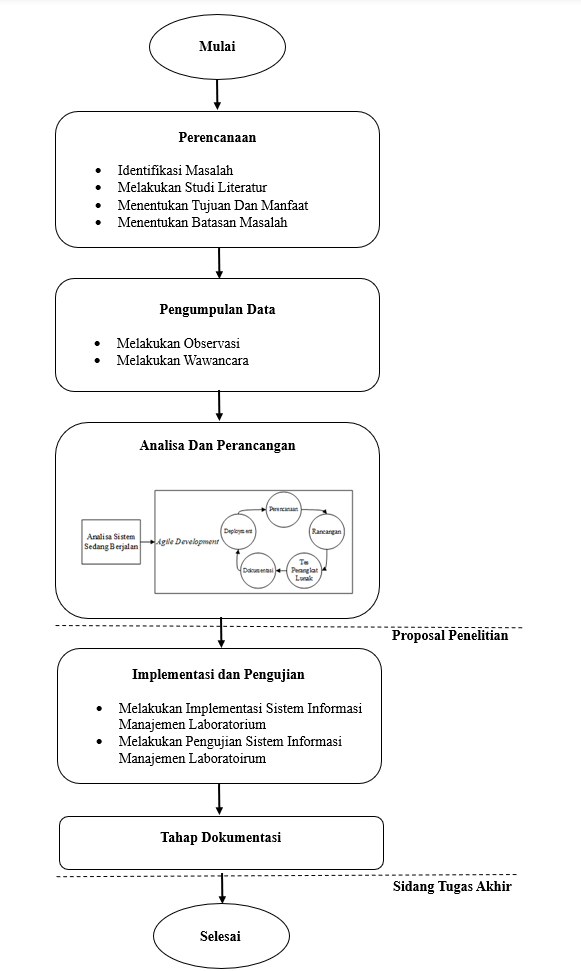
\includegraphics[width=0.82\linewidth]{konten//gambar/metodologi-penelitian.png}
	\caption{Metodologi Penelitian}
	\label{fig:enter-label}
\end{figure}
%-----------------------------------------------------------------------------%


